\documentclass[../review_1.tex]{subfiles}
\graphicspath{{\subfix{../img/}}}
\begin{document}
\chapter{Risikoanalyse}\thispagestyle{fancy}
\section{Risikoidentifikation}
Durch Befragung des gesamten Projektteams wurden sowohl fachliche, kaufmännische und planerische Risiken identifiziert. Indem Teammitglieder mit unterschiedlichen Erfahrungen und Fachkompetenzen miteinbezogen wurden, konnten Risiken aus verschiedenen Blickwinkeln identifiziert werden. In der folgenden Tabelle werden sowohl die verschiedenen Risiken als auch deren Eintrittswahrscheinlichkeit\footnote{Wert zwischen 0\% und 100\%. 0\% entspricht dem unmöglichen Ereignis, 100\% dem sicheren Ereignis. Ereignisse mit Werten nahe 0\% sind unwahrscheinlich, Ereignisse mit Werten nahe 100\% wahrscheinlich.}, Auswirkung und Maßnahmen kurz beschrieben.\\ Die dort beschriebenen Maßnahmen verfolgen das Ziel, die Eintrittswahrscheinlichkeit zu verringern und bei Eintritt die Auswirkungen abzuschwächen.\\
\textbf{Hinweis}: Die unten stehenden Tabelle wird im Laufe des Projektes noch weiter ergänzt, da die Risikoanalyse keine einmalige, sondern fortlaufende Aktivität im Projekt darstellt. So können beispielsweise neue Risiken auftauchen, die zu Beginn des Projektes noch nicht vorhanden waren oder übersehen wurden. Auch Eintrittswahrscheinlichkeiten können sich noch ändern. Außerdem ist es möglich, dass Auswirkungen und Maßnahmen hinzukommen oder verschwinden.

\begin{longtable}[h]{l p{2,5cm} p{2,5cm} p{3,5cm} p{3,5cm}}
    \textbf{ID} & \textbf{Risiko}                                                                                                                                           & \textbf{Eintrittswahr-scheinlichkeit} & \textbf{Auswirkung}                                                                                                                                                                                       & \textbf{Maßnahmen}                                                                                                                                                                                                           \\ \toprule \endhead
    R01         & Software wird unzureichend dokumentiert.                                                                                                                  & 30\%                                  & Sicherheitslücken, falsch aufgefasste Anforderungen, Softwareanomalien, schwierige Wartung, Software kann nicht richtig getestet werden u. v. m.                                                          & Motivation der Teammitglieder dazu, dass diese gewissenhaft Dokumentation führen; Erklären der Wichtigkeit der Dokumentation; Einführen von Konventionen zur Dokumentation; Verwendung automatischer Dokumentationswerkzeuge \\
    R02         & Unzureichende Erfahrung des Projektteams bezüglich neuer Tools (z. B. DPDK, Ninja, Meson) und der Programmiersprache C++                                  & 80\%                                  & Zeitverzögerung (v. a. längere Dauer der Implementierung durch umfassende Einarbeitungsphase)                                                                                                             & Gute Einarbeitung; Erstellen und Halten von Präsentationen zu schwierigen Themen; Gegenseitige Hilfe; Festlegen von Ansprechpartner für die einzelnen Themenbereiche                                                         \\
    R03         & Weniger Austausch und weniger effiziente Zusammenarbeit durch  Online-Lehre                                                                               & 70\%                                  & Probleme werden später oder nicht sichtbar; schwieriger Überblick über den Arbeitsstand bei anderen Teammitgliedern; Statusmeldungen fehlen; Geringes Teamgefühl                                          & regelmäßige Treffen ohne Zeitdruck; möglichst organisierte Kommunikation (z.B. über Zulip oder Webex)                                                                                                                        \\
    R04         & Hardware-Probleme (z. B. Ausfall oder andere Defekte)                                                                                                     & 20\%                                  & Zeitverzögerung, finanzielle Kosten                                                                                                                                                                       & sorgfältiger Umgang mit der Hardware                                                                                                                                                                                         \\
    R05         & Testbed nicht optimal konfigurierbar (aufgrund der verringerten Geräteanzahl und beschränkter Optionen ist nicht jede vorteilhafte Konstellation möglich) & 60\%                                  & erschwerte Implementierung, Zeitverzögerung, Nichterfüllen einzelner Anforderungen, finanzielle Kosten beim Kauf zusätzlicher Hardware & möglichst effiziente Nutzung der vorhandenen Hardware; Kauf zusätzlicher Hardware; Entwicklung eines Netzwerkplans                                                                                                           \\
\end{longtable}

\section{Risikomatrix}
\noindent Die folgende Risikomatrix (auch Risikoportfolio, Risikodiagramm oder Risiko-Map, siehe Abbildung 5.1) visualisiert die Projektrisiken R01 bis R06, indem sie die Eintrittswahrscheinlichkeiten und die dazugehörigen Schadensausmaße ins Verhältnis setzt. Je weiter man sich im Diagramm nach rechts bewegt, desto höher ist die Eintrittswahrscheinlichkeit. Während diese Wahrscheinlichkeit ganz links bei 0\% liegt, beträgt sie am rechten Rand 100\%. Je weiter oben sich das Risiko im Diagramm befindet, desto größer ist das Schadensausmaß.\\
Bei den Risiken, die sich im grünen Bereich befinden, sind keine zusätzlichen Maßnahmen zur Risikominimierung notwendig, wohingegen die Risiken im gelben Bereich so weit wie möglich abgemindert werden sollen. Die gefährlichsten Risiken befinden sich im roten Bereich. Für diese Risiken müssen geeignete Präventionsmaßnahmen getroffen werden, um sie in den gelben Bereich zu bewegen.\\
Ebenso kann man aus der Position der Risiken ableiten, wie dringend Präventionsmaßnahmen eingeführt werden müssen.\\
\begin{figure} [h]
    \centering
    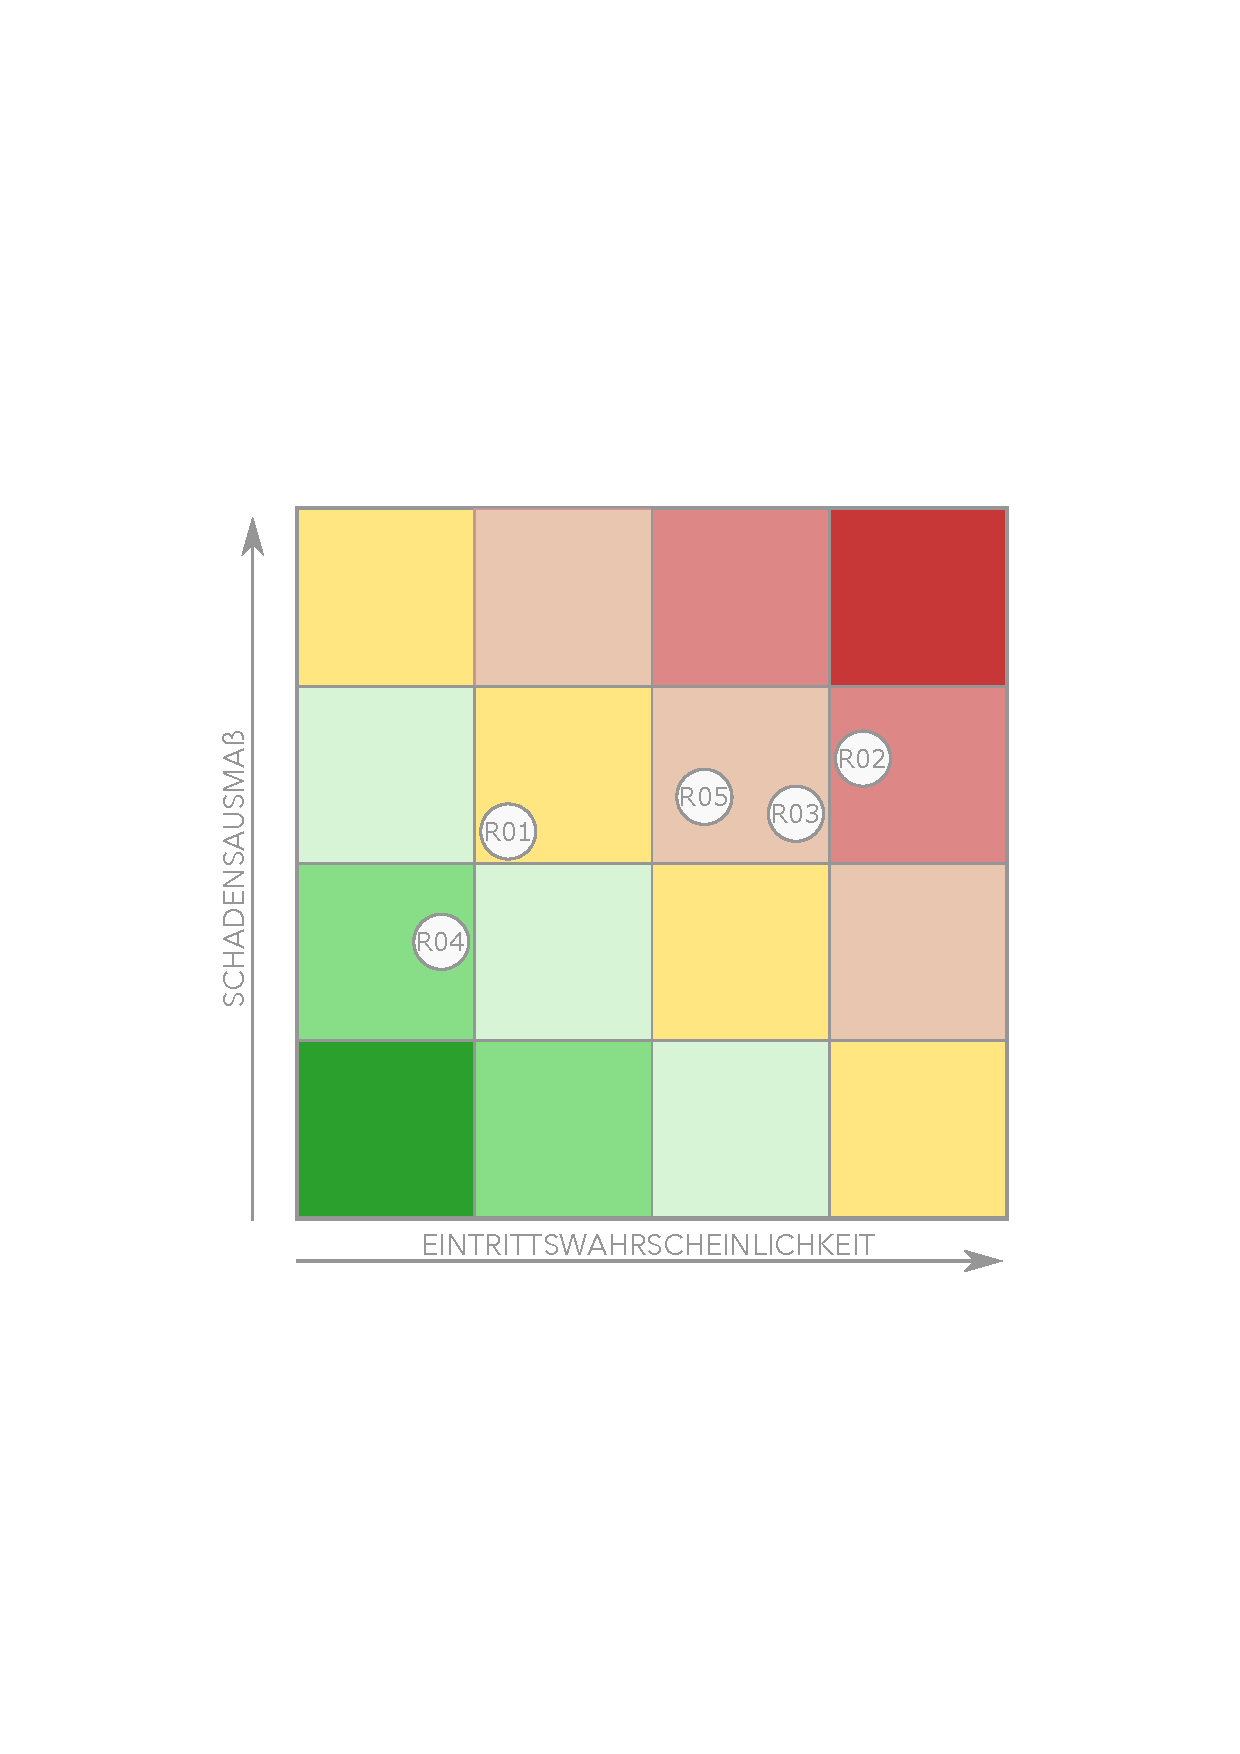
\includegraphics[width=9cm]{risikomatrix.pdf}
    \caption{Risikomatrix mit den Risiken R01 bis R06}
\end{figure}
\\ \newline Aus der Grafik lässt sich erkennen, dass vor allem für die Risiken R02, R03 und R05 geeignete Maßnahmen zur Minimierung der Risiken eingeführt werden müssen.

\section{Verbindung zum Vorgehensmodell}
Indem sich für den Unified Process als Vorgehensmodell entschieden wurde, werden in dem Projekt Risiken schon frühzeitig adressiert. Zudem werden zu Beginn jeder Phase jeweils die Punkte mit den größten Risiken zuerst bearbeitet.

\end{document}
